% !TeX program = pdflatex
% !BIB program = bibtex
% Template LaTeX file for DAFx-19 papers

%------------------------------------------------------------------------------------------
%  !  !  !  !  !  !  !  !  !  !  !  ! user defined variables  !  !  !  !  !  !  !  !  !  !  !  !  !  !
% Please use these commands to define title and author(s) of the paper:
\def\papertitle{Complex Nonlinearities for Audio Signal Processing}
\def\paperauthorA{Jatin Chowdhury}

% Authors' affiliations have to be set below

%------------------------------------------------------------------------------------------
\documentclass[twoside,a4paper]{article}
\usepackage{dafx_19}
\usepackage{amsmath,amssymb,amsfonts,amsthm}
\usepackage{euscript}
\usepackage[latin1]{inputenc}
\usepackage[T1]{fontenc}
\usepackage{ifpdf}

\usepackage[english]{babel}
\usepackage{caption}
\usepackage{subfig} % or can use subcaption package
\usepackage{xcolor}

\setcounter{page}{1}
\ninept

\usepackage{times}
% Saves a lot of ouptut space in PDF... after conversion with the distiller
% Delete if you cannot get PS fonts working on your system.

% pdf-tex settings: detect automatically if run by latex or pdflatex
\newif\ifpdf
\ifx\pdfoutput\relax
\else
   \ifcase\pdfoutput
      \pdffalse
   \else
      \pdftrue
\fi

\ifpdf % compiling with pdflatex
  \usepackage[pdftex,
    pdftitle={\papertitle},
    pdfauthor={\paperauthorA},
    colorlinks=false, % links are activated as colror boxes instead of color text
    bookmarksnumbered, % use section numbers with bookmarks
    pdfstartview=XYZ % start with zoom=100% instead of full screen; especially useful if working with a big screen :-)
  ]{hyperref}
  \pdfcompresslevel=9
  \usepackage[pdftex]{graphicx}
  \usepackage[figure,table]{hypcap}
\else % compiling with latex
  \usepackage[dvips]{epsfig,graphicx}
  \usepackage[dvips,
    colorlinks=false, % no color links
    bookmarksnumbered, % use section numbers with bookmarks
    pdfstartview=XYZ % start with zoom=100% instead of full screen
  ]{hyperref}
  % hyperrefs are active in the pdf file after conversion
  \usepackage[figure,table]{hypcap}
\fi

% My packages
\usepackage{tikz}
\usetikzlibrary{dsp,chains}
\usepackage{tkz-euclide}
\usetkzobj{all}
\usepackage{cleveref}

\usepackage{listings}
\definecolor{codegreen}{rgb}{0,0.6,0}
\definecolor{codegray}{rgb}{0.5,0.5,0.5}
\definecolor{codepurple}{rgb}{0.58,0,0.82}
\definecolor{backcolour}{rgb}{0.95,0.95,0.92}
 
\lstdefinestyle{mystyle}{
    backgroundcolor=\color{backcolour},   
    commentstyle=\color{codegreen},
    keywordstyle=\color{magenta},
    numberstyle=\tiny\color{codegray},
    stringstyle=\color{codepurple},
    basicstyle=\footnotesize,
    columns=flexible,
    breakatwhitespace=false,         
    breaklines=true,                 
    captionpos=b,                    
    keepspaces=true,                               
    showspaces=false,                
    showstringspaces=false,
    showtabs=false,                  
    tabsize=4
}
 
\lstset{style=mystyle}

\DeclareMathAlphabet{\mathpzc}{OT1}{pzc}{m}{it}
\newcommand{\z}{\mathpzc{z}}

\title{\papertitle}

\affiliation{
\paperauthorA \,}
{\href{http://ccrma.stanford.edu}{Center for Computer Research in Music and Acoustics} \\ Stanford University \\ Palo Alto, CA \\ {\tt \href{mailto:jatin@ccrma.stanford.edu}{jatin@ccrma.stanford.edu}}}

\begin{document}
% more pdf-tex settings:
\ifpdf % used graphic file format for pdflatex
  \DeclareGraphicsExtensions{.png,.jpg,.pdf}
\else  % used graphic file format for latex
  \DeclareGraphicsExtensions{.eps}
\fi

\maketitle
%
\begin{abstract}
In this writing, we present an ongoing study of new and interesting
nonlinear structures for audio signal processing, intended to be
used for audio effects and synthesis. We give a brief discussion of
each structure, and present a series of open-source audio plugins that
implement the structures.
\end{abstract}

\section{Introduction} \label{sec:intro}
%
In digital audio signal processing it is common to find audio effects
that use nonlinear elements to add harmonic content to the signal being
processed, or to achieve a ``distortion'' type of effect. Typically, this
is done either as part of an analog model, or using a static memoryless
nonlinear element.
\newline\newline
%
The goal of this research project is to develop structures for nonlinear
audio signal processing that go beyond the traditionally used simple
nonlinearities. While the structures developed here may be used for
analog modelling and may be inspired by analog effects, they do not
come about from direct physical modelling of an analog system, nor
do they require knowledge of analog systems such as circuits to be
understood and implemented.

\subsection{Simple Nonlinearities} \label{sec:simple}
%
We refer to the desired nonlinear structures as ``Complex
Nonlinearities'', as such we should take a moment to define what
constitutes a ``simple'' nonlinearity, particularly since these will
make up the building blocks of the complex nonlinearities that follow.

\subsubsection{Saturators} \label{sec:sat}
%
The most commonly used nonlinearity in audio signal processing is
the saturating nonlinearity, where the input ``clips'' to a constant
value as the input gain increases. This class of nonlinearity includes
functions such as the hard clipper, cubic soft clipper, and $tanh$
nonlinearities \cite{Yeh}, which are described by the following functions:
%
\begin{equation}
    f_{\text{hard clip}}(x) = \begin{cases}
        -1& x < -1 \\
        x& -1 \leq x \leq 1 \\
        1& x > 1
    \end{cases}
    \label{eq:hard-clip}
\end{equation}
\newline
%
\begin{equation}
    f_{\text{soft clip}}(x) = \begin{cases}
        -\frac{2}{3}& x < -1 \\
        x - \frac{x^3}{3}& -1 \leq x \leq 1 \\
        \frac{2}{3}& x > 1
    \end{cases}
    \label{eq:soft-clip}
\end{equation}
\newline
%
\begin{equation}
    f_{\text{tanh}}(x) = \tanh(x)
    \label{eq:tanh-clip}
\end{equation}
%
\begin{figure}[h]
    \center
    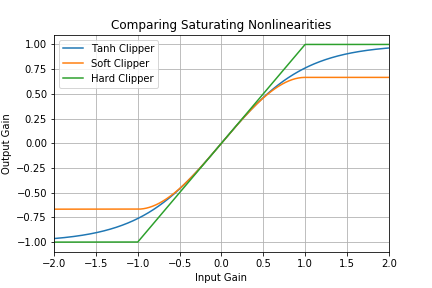
\includegraphics[width=3in]{../NonlinearBiquad/Pics/Sat-NLs.png}
    \caption{\label{Sats}{\it Saturating Nonlinearities}}
\end{figure}
%

\subsubsection{Rectifiers} \label{sec:rect}
%
Sometimes for audio effects such as compressors and limiters, it is
useful to have a rectified signal (i.e. a signal that only contains
non-negative values). The two most simple rectifying nonlinearities
are the full-wave rectifier and the half-wave rectifier:
%
\begin{equation}
    f_{\text{FWR}}(x) = |x|
    \label{eq:fwr}
\end{equation}
%
\begin{equation}
    f_{\text{HWR}}(x) = \begin{cases}
        0& x < 0 \\
        x& x \geq 0
    \end{cases}
    \label{eq:hwr}
\end{equation}
%
The above rectifier equations have a downside in that they don't have
continuous derivatives. As a substitute we present an alternate
half-wave rectifier equation loosely modelled from a Shockley diode
rectifier:
\begin{equation}
    f_{\text{Diode}}(x) = \beta \left(e^{\alpha x} - 1 \right)
    \label{eq:diode}
\end{equation}
%
where $\alpha$ and $\beta$ are tunable parameters.
%
\begin{figure}[h]
    \center
    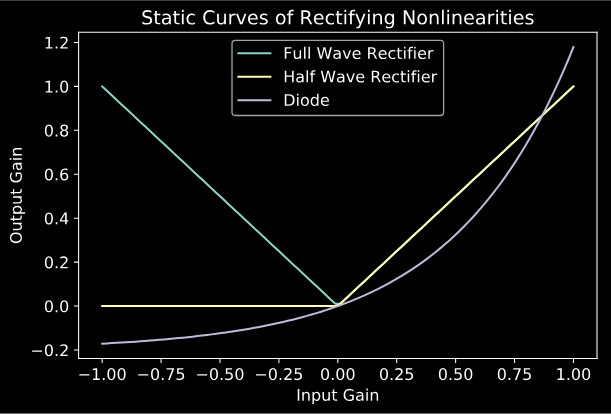
\includegraphics[width=3in]{../Exciter/Pics/rect_static.png}
    \caption{\label{Rects}{\it Rectifying Nonlinearities. For the diode nonlinearity,
    we use $\beta = 0.2$, $\alpha = 1.93$.}}
\end{figure}
%
\begin{figure}[h]
    \center
    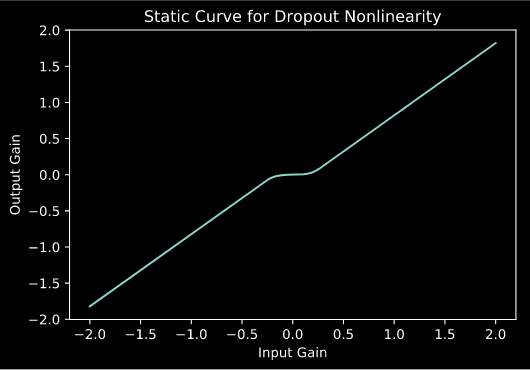
\includegraphics[width=3in]{Pics/dropout.png}
    \caption{\label{Drops}{\it Dropout nonlinearity with $a = 0.6$.}}
\end{figure}
%

\subsubsection{Dropout} \label{sec:drop}
%
Another nonlinearity used in audio effects is the ``dropout'' nonlinearity,
notably used for modelling underbiased analog tape recording \cite{DAFX-tape}.
A dropout nonlinearity is characterized by the fact that small input values
are snapped to zero. Here we present a simple cubic dropout function:
%
\begin{equation}
    f_{\text{Dropout}}(x) = \begin{cases}
        x + B - \left(\frac{B}{a}\right)^3& x < -B \\
        \left(\frac{x}{a}\right)^3& -B \leq x \leq B \\
        x - B + \left(\frac{B}{a}\right)^3& x > B
    \end{cases}
    \label{eq:dropout}
\end{equation}
%
where $a$ is a tunable parameter, and $B = \sqrt{\frac{a^3}{3}}$.
%

\section{Double Soft Clipper} \label{sec:DSC}
%
The Double Soft Clipper (see \cref{DSC}) is a sort of
combination between a saturating nonlinearity and dropout
nonlinearity. The nonlinear function is given as:
%
\begin{equation}
    f_{\text{DSC}}(x) = \begin{cases}
        1 & u \geq 1 \\
        (3/4) * (u - u^3/3) + 0.5 & 0 < u < 1 \\
        (3/4) * (u - u^3/3) - 0.5 & -1 < u < 0 \\
        -1 & u \leq -1
    \end{cases}
    \label{eq:double-soft-clip}
\end{equation}
%
where
%
\begin{equation}
    u(x) = \begin{cases}
    x - 0.5 & x > 0 \\
    x + 0.5 & x < 0
    \end{cases}
    \label{eq:double-soft-clip_u}
\end{equation}
%
The resulting static curve is essentially two cubic soft
clipping functions stacked on top of each other (see \cref{DSC-stack}).
%
\begin{figure}[h]
    \center
    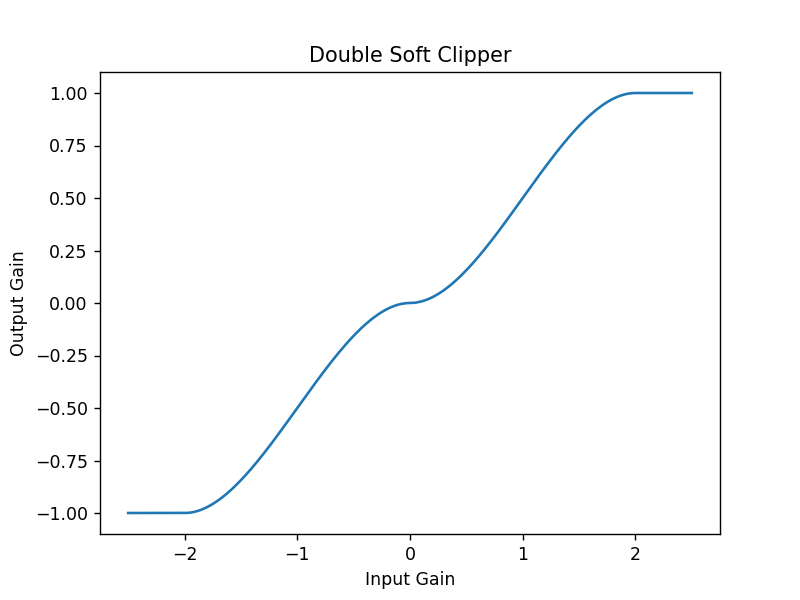
\includegraphics[width=3in]{../DoubleSoftClipper/Pics/Double.png}
    \caption{\label{DSC}{\it Double soft clipper.}}
\end{figure}
%
\begin{figure}[h]
    \center
    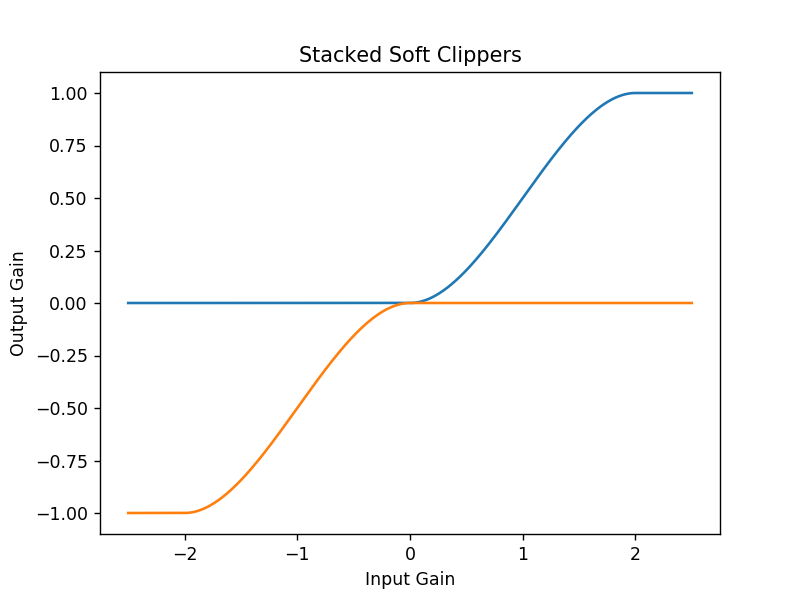
\includegraphics[width=3in]{../DoubleSoftClipper/Pics/stacked.png}
    \caption{\label{DSC-stack}{\it Stacked soft clippers.}}
\end{figure}
%
One advantage of this nonlinear function is that it is highly
parameterizable. Possible parameters include upper/lower clipping
limit, linear slope, upper/lower skew,  and dropout width (see
\cref{DSCs}).
%
\begin{figure*}[ht]
    % \center
    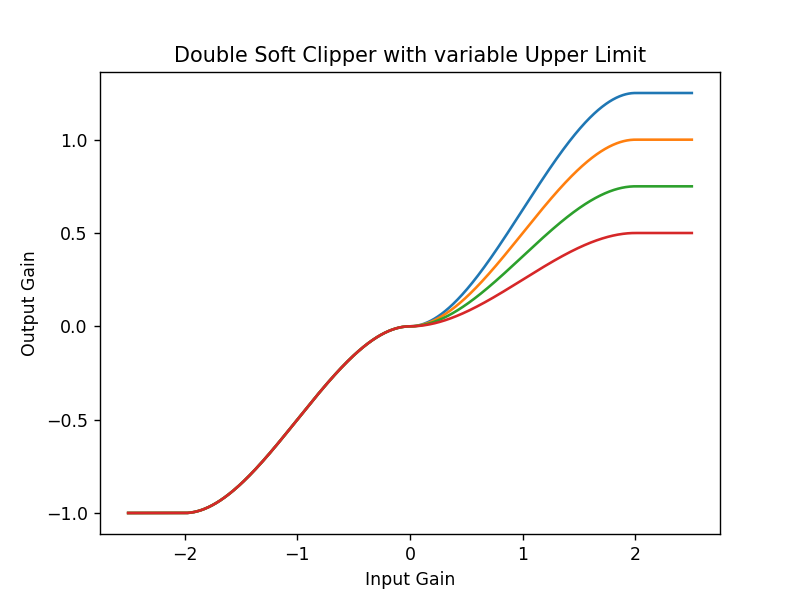
\includegraphics[width=2.2in]{../DoubleSoftClipper/Pics/VarUpperLim.png}
    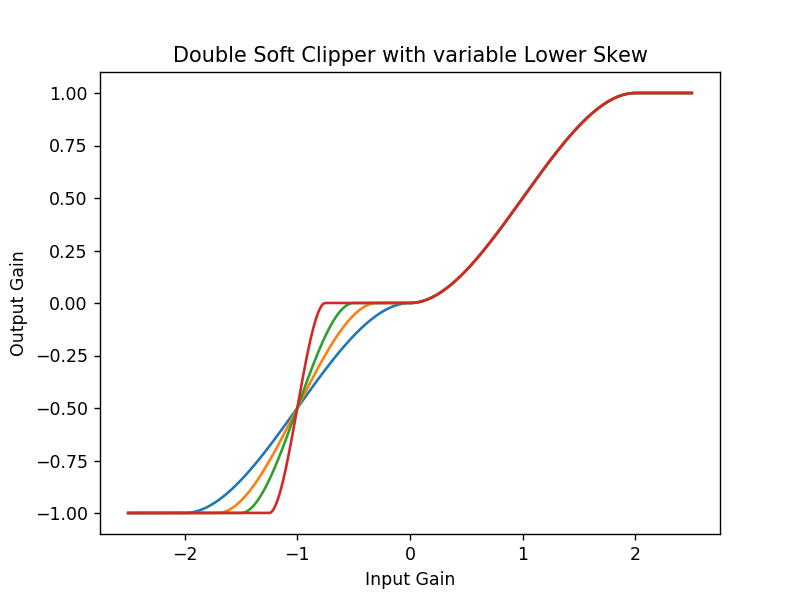
\includegraphics[width=2.2in]{../DoubleSoftClipper/Pics/VarLowSkew.png}
    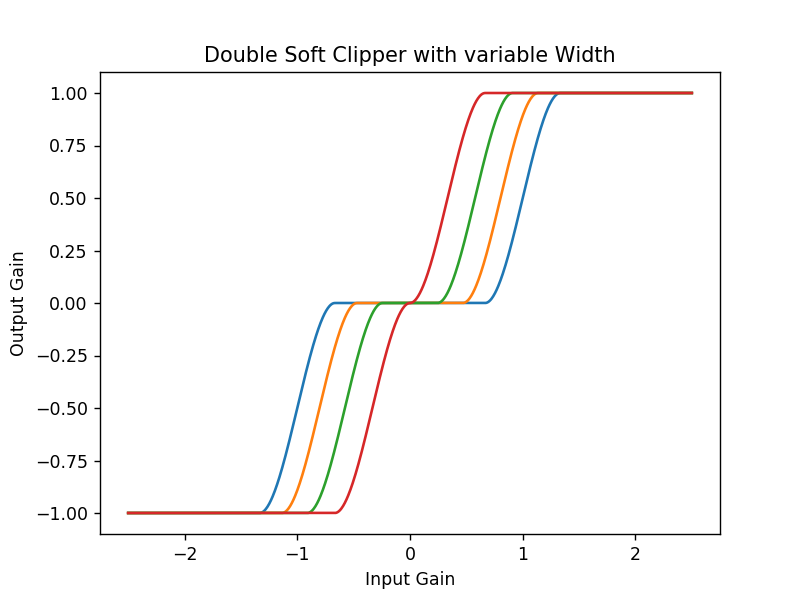
\includegraphics[width=2.2in]{../DoubleSoftClipper/Pics/VarWidth.png}
    \caption{\label{DSCs}{\it Double soft clippers with variable upper clipping
    limit (left), variable lower skew (middle), and variable dropout width (right).}}
\end{figure*}
%
\section{Harmonic Exciter} \label{sec:exciter}
%
A harmonic exciter is an audio effect often used by mixing
engineers to add ``brightness'' to a track or a mix, for example
the Aphex Aural Exciter \cite{aphex}. Typically, digital exciter effects
are implemented as circuit models of an original analog effect (e.g.
\cite{exciter-model}). The goal of this work is to create a
generalized exciter model that can be implemented without knowledge of
circuit theory, much in the way that \cite{giannoulis2012digital} describes
a generalized model of a dynamic range compressor.
\newline\newline
Based loosly on the Aphex Aural Exciter, we propose the
exciter architecture shown in \cref{exc}. For the generator
component, we propose the processing architecture shown in
\cref{gen}.
\newline\newline
For the level detector component, we propose using a rectifying
nonlinearity followed by a lowpass filter. \Cref{detect} shows the
output of a level detector with the rectifying nonlinearities described
in \S\ref{sec:rect} and a first-order lowpass filter with a cutoff
frequency of 10 Hz. For the nonlinearity component, any saturating
nonlinearity of the type described in \S\ref{sec:sat} will suffice. The
output of the generator is very harmonically rich, with both even and odd
harmonics, as seen in \cref{exc-harm}.
\newline\newline
%
\begin{figure}[h]
    \center
    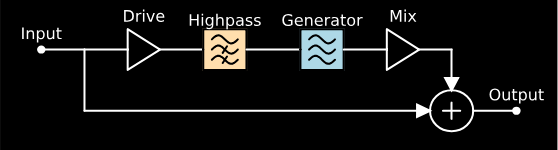
\includegraphics[width=3in]{../Exciter/Pics/Exciter_FullArch.png}
    \caption{\label{exc}{\it Exciter architecture.}}
\end{figure}
%
\begin{figure}[h]
    \center
    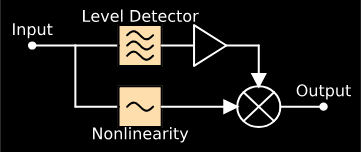
\includegraphics[width=3in]{../Exciter/Pics/Exciter_Arch.png}
    \caption{\label{gen}{\it Exciter generator architecture.}}
\end{figure}
%
\begin{figure}[h]
    \center
    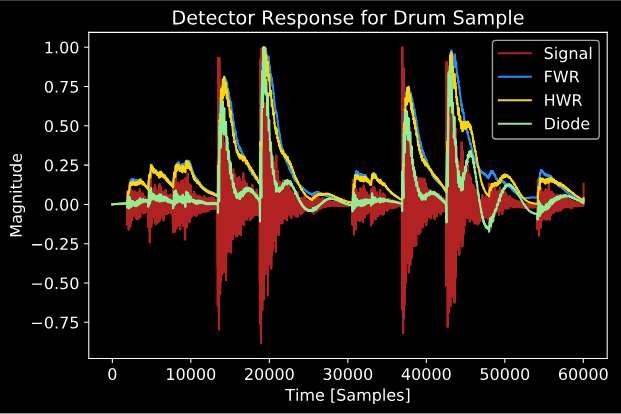
\includegraphics[width=3in]{../Exciter/Pics/Waveform_Detected.png}
    \caption{\label{detect}{\it Exciter level detector.}}
\end{figure}
%
\begin{figure*}[ht]
    % \center
    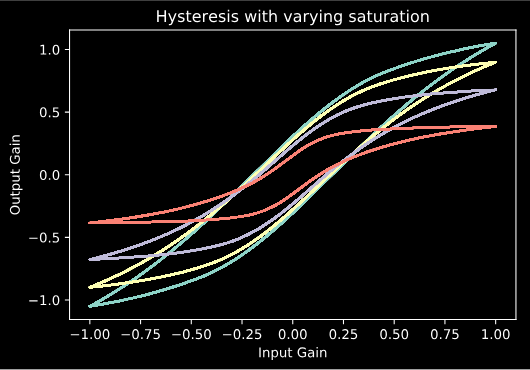
\includegraphics[width=2.2in]{../Hysteresis/Pics/Saturations.png}
    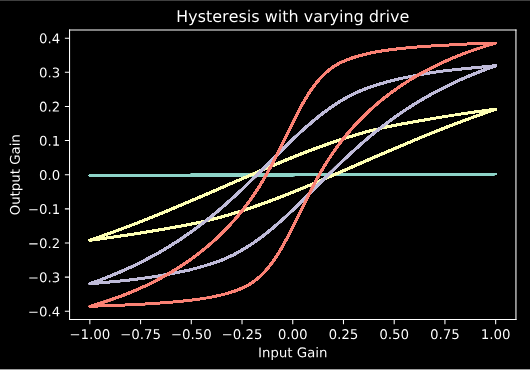
\includegraphics[width=2.2in]{../Hysteresis/Pics/Drive.png}
    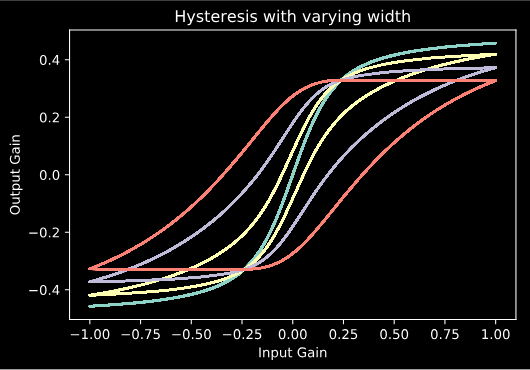
\includegraphics[width=2.2in]{../Hysteresis/Pics/Width.png}
    \caption{\label{hysteresis}{\it Hysteresis curves with variable saturation
    (left), drive (middle), and width (right).}}
\end{figure*}
%
\begin{figure}[h]
    \center
    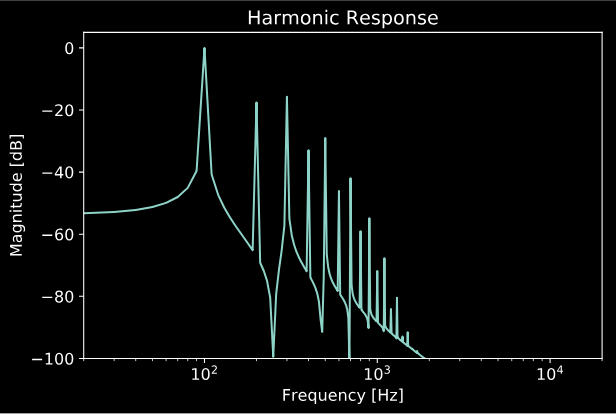
\includegraphics[width=3in]{../Exciter/Pics/exciter_harm.png}
    \caption{\label{exc-harm}{\it Exciter generator harmonic response.}}
\end{figure}
%
\section{Hysteresis} \label{sec:hysteresis}
%
Hysteresis is an interesting complex nonlinear behavior
that describes the magnetising of magnetic materials, as
well as concepts in other fields including chemistry, structural engineering,
even economics. \cite{DAFX-tape} uses an adaptation of the Jiles-Atherton
magnetic hysteresis model to recreate the sound of an analog tape machine.
In this study, we attempt to generalize this hysteresis model to be used
and implemented without understanding of electromagnetic physics,
as well as adding useful parameters to the hysteresis nonlinearity.
\newline\newline
%
The hysteresis model for input $x$ is defined by the differential equation:
%
\begin{equation}
    \dot{y} = \frac{\frac{(1-c)\delta_y(SL(Q) - y)}{(1-c)\delta_xk - \alpha(SL(Q) - y)}\dot{x} + c \frac{S}{a} \dot{x} L'(Q)}{1 - c\alpha \frac{S}{a} L'(Q)}
    \label{eq:hysteresis}
\end{equation}
%
where $\dot{y}$ denotes the time derivative of the output, and $k$ and
$a$ are constant values. $\delta_x$ and $\delta_y$ are defined as
%
\begin{equation}
    \delta_x = \begin{cases} 1 & \text{if $x$ is increasing} \\ -1 & \text{if $x$ is decreasing} \end{cases}
    \label{eq:delta-x}
\end{equation}
%
\begin{equation}
    \delta_y = \begin{cases} 1 & \text{if $\delta_x$ and $L(Q) - y$ have the same sign} \\ 0 & \text{otherwise} \end{cases}
    \label{eq:delta-y}
\end{equation}
%
$L(x)$ denotes the Langevin function:
%
\begin{equation}
    L(x) = \coth(x) - \frac{1}{x}
    \label{eq:langevin}
\end{equation}
%
and $Q$ is defined as
%
\begin{equation}
    Q(x,y) = \frac{x + \alpha y}{a}
    \label{eq:hyst-q}
\end{equation}
%
where $\alpha$ is a constant value, and $x$ and $y$ are the system input
and output respectively.
\newline\newline
The variables $S$, $a$, and $c$ from \cref{eq:hysteresis} can be used
as parameters to control the hysteresis function saturation, drive,
and width respectively. \Cref{hysteresis} shows the effects of modulating
these parameters.

\section{Nonlinear Biquads} \label{sec:nlbq}
%
Transposed Direct Form II (TDF-II) (see \cref{tdf2}) is a standard method for
implementing biquad filters in signal processing. We present two
methods for adding nonlinear elements to the TDF-II structure that
can create interesting sonic effects without affecting the filter's
stability.
\newline\newline
For the first method we propose adding nonlinear elements before the delay
elements in the filter structure, as shown in \cref{nlbq}. When saturating
nonlinearities are used for these elements, the filter exhibits ``nonlinear
resonance'' similar to many analog filters. The filter frequency response at
various operating points is shown in \cref{nlbq-lpf}.
\newline\newline
For the second method we propose adding nonlinear elements to the feedback
paths of the filter, as shown in \cref{nlfd}. Again, with saturating
nonliearities, this structure causes the filter poles to ``sweep'' to
different frequencies as the input level of the filter varies. The filter
frequency response at various operating points is shown in \cref{nlfd-lpf}.
\newline\newline
In order to maintain stability, we propose that the nonlinear elements must
satisfy the constraint that $|f'_{NL}(x)| \leq 1$ (note that this implies that
the derivative of the nonlinear function must exist everywhere in the range
of $x$). A proof of this constraint using Lyapunov stability, as well as a
more in-depth analysis of these nonlinear filter structures, including the
potential use of these structures for analog modelling, is given in
\cite{NLBiquad}.
%
\begin{figure}[h]
    \center
    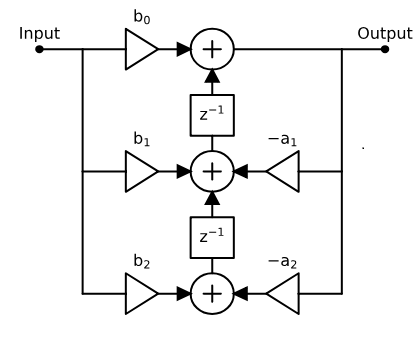
\includegraphics[width=3in]{../NonlinearBiquad/Pics/TDF-II-White.png}
    \caption{\label{tdf2}{\it Transposed direct form II filter structure.}}
\end{figure}
%
\begin{figure}[h]
    \center
    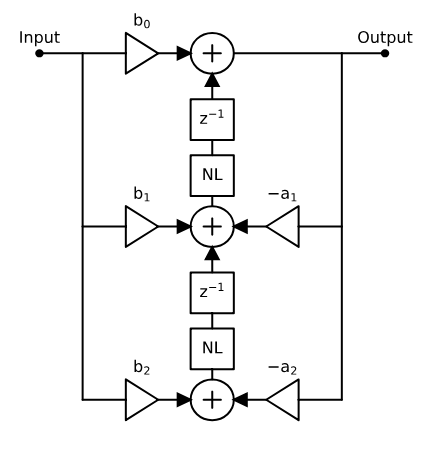
\includegraphics[width=3in]{../NonlinearBiquad/Pics/NL-TDF-II-White.png}
    \caption{\label{nlbq}{\it Transposed direct form II with nonlinear resonance.}}
\end{figure}
%
\begin{figure}[h]
    \center
    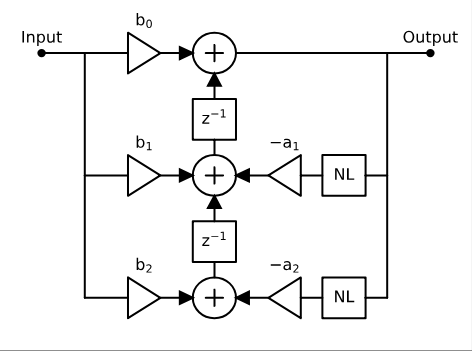
\includegraphics[width=3in]{../NonlinearFeedback/Pics/NL2-TDF-II-White.png}
    \caption{\label{nlfd}{\it Transposed direct form II with nonlinear feedback.}}
\end{figure}
%
\begin{figure}[h]
    \center
    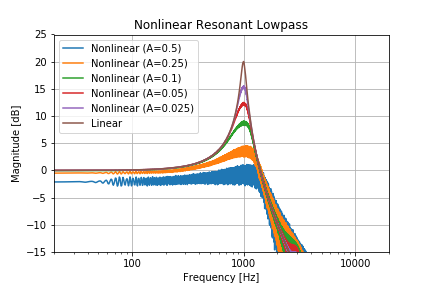
\includegraphics[width=3in]{../NonlinearBiquad/Pics/NL-LPF.png}
    \caption{\label{nlbq-lpf}{\it Frequency response of nonlinear resonance filter at
    various operating points.}}
\end{figure}
%
\begin{figure}[h]
    \center
    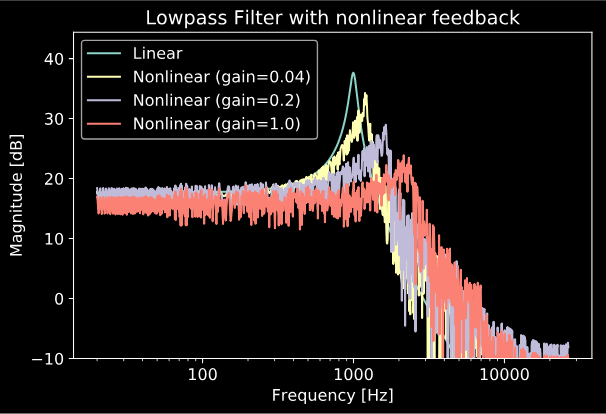
\includegraphics[width=3in]{../NonlinearFeedback/Pics/LPF-NL.png}
    \caption{\label{nlfd-lpf}{\it Frequency response of nonlinear feedback filter at
    various operating points.}}
\end{figure}
%

\section{Implementation and Presentation} \label{sec:pres}
%
The work done in this study was designed to be informative and inspiring
both to recording engineers and musicians, as well as programmers and
aspiring DSP engineers looking to design audio effects. With this audience
in mind, it was determined that the results of this work should be written
and presented for a relatively non-technical reader, and published in a
location where these readers would most easily find it. To that end, the
results of this work have been published as a series of articles on the
popular blog website Medium \footnote{https://medium.com/@jatinchowdhury18}.
According to statistics on the site, the articles have been read approximately
300 times as of this writing. Additionally, the structures developed
in this study have been implemented as a series of audio plugins using JUCE/C++.
The plugins and their source code are freely available on GitHub
\footnote{https://github.com/jatinchowdhury18/ComplexNonlinearities}.

\section{Conclusion} \label{sec:conclusion}
%
In this paper, we have presented a series of complex nonlinear signal
processing structures, with the intention of being used for audio effects
and synthesis software. While this work has developed a number of useful
and sonically rich structures, there is great potential for many more
developements in this area of audio signal processing. We look forward
to seeing more audio effects being built using these methods, as well as to
more nonlinear DSP methods being developed in the vein of this work.

\section{Acknowledgments}
%
The author would like to thank Julius Smith, Kurt Werner, Viraga Perera,
Dave Berners, and the GASP working group for providing inspiring discussions
and indispensible feedback.

%\newpage
\nocite{*}
\bibliographystyle{IEEEbib}
\bibliography{references}

\end{document}
